\scanpage{130}
\mspage{V.1}
% archive sheet number: 129

% L01-03 title and superposed title
\uline{IV}

\inserted{\uline{Propriétés générales des faisceaux de cycles évanescents.}}
\deleted{\unsure{Les}} \uline{Cas des points singuliers isolés de la fibre spéciale.}

% L04-06
\uline{1.} Calcul \deleted{\unsure{des}}\inserted{de \deleted{\unsure{leur}} la} \unsure{fibre|fibres} des faisceaux des cycles évanescents, \deleted{\unsure{en}}\inserted{comme} \deleted{\unsure{terme} de la} cohomologie de la fibre générique géométrique d'un localisé strict.

% L07-15 note enclosed by an oval, in the left middle of the sheet
\margin{\figure{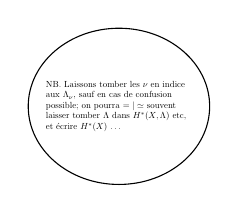
\begin{tikzpicture}[scale=.32,transform shape]
\draw (0,0) ellipse (3.6cm and 3.1cm);
\node[text width=5.8cm,align=left] at (0,0) {\uline{NB.} Laissons tomber les $\nu$ en indice aux $\Lambda_\nu$, sauf en cas de confusion possible; on pourra $\unsure{=|\simeq}$ souvent laisser tomber $\Lambda$ dans $H^*(X,\Lambda)$ etc, et écrire $H^*(X)$ \ldots};
\end{tikzpicture}}}
